\secput{algo}{An Exact Algorithm for the code-clone selection puzzle}

Now, let's describe an exact algorithm to solve the puzzle. Since if $k
= m$, or $k = m-1$, the solution is trivial, in the following algorithm
description, let's assume that $k \leq m-2$.

The algorithm can be roughly divided into two stages:

\begin{enumerate}

    \item Establish a hierarchical {DAG} out of the $m$ input columns 

    \item Calculate the $k$-medians (unified by $\otimes$ operation)
    \footnote{In the rest of this document, we use the term ``median'' and
    ``unified column'' interchangably}and the optimal values out of the
    hierarchical {DAG}

\end{enumerate}
    
Before the description of algorithm, let's define some notations that will
be used throughout the text: for the original set of $m$ input columns,
let's denote it as $\mathcal{C} = \{ c_0, c_1, \ldots, c_{m-1} \}$, for
all nodes derived from input columns and construct the hierarchical {DAG}
$T$, we denote it as $\mathcal{V} = \{ v_0, v_1, \ldots, v_{M-1} \}$,
where $M$ is the total number of nodes in the {DAG}.  Apparently,
$\mathcal{C} \subseteq \mathcal{V}$. For each node $v_i \in \mathcal{V}$,
we denote the sub-tree rooted at $v_i$ to be $T_{v_i}$, the set of original
input columns to be $\mathcal{C}_i$, the set of total nodes to be 
$\mathcal{V}_i$, and $\mathcal{C}_i \subseteq \mathcal{V}_i$ holds.
Correspondingly, we denote the set of $k$-medians as $\mathcal{M} =
\{m_0, m_1, \ldots, m_{k-1}\}$.  The sub-tree rooted at a median $m_i$
to be $T_{m_i}$ The set of original input columns and total nodes are
denoted as $\mathcal{C}_{m_i}$ and $\mathcal{V}_{m_i}$, respectively.

\subsecput{stage1}{Construct a hierarchical {DAG}}
In stage $1$, we need to construct a hierarchical {DAG}, denoted as $T$
out of the $m$ input columns. The entire procedure is a dynamic programming.

\begin{figure}[!ht]
\begin{minipage}[b]{0.3\linewidth}
\centering
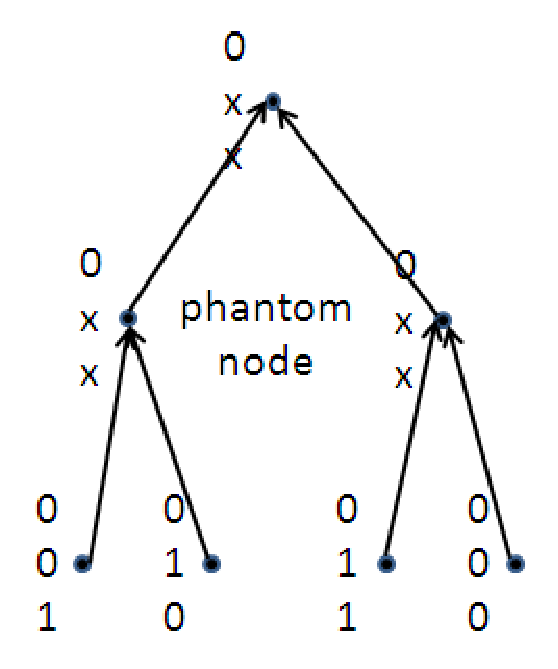
\includegraphics[scale=0.5]{figures/phantom_node.eps}
\caption{Phantom Nodes}
\label{fig:phantom-node}
\end{minipage}
\hspace{0.1cm}
\begin{minipage}[b]{0.3\linewidth}
\centering
\begin{tabular}{c|ccc}
$\otimes$ & 0 & 1 & x \\
\hline 
0 & 0 & x & x \\
1 & x & 1 & x \\
x & x & x & x 
\end{tabular}
\caption{Truth table for $\otimes$ operation}
\label{fig:truth-table}
\end{minipage}
\hspace{0.1cm}
\begin{minipage}[b]{0.3\linewidth}
\centering
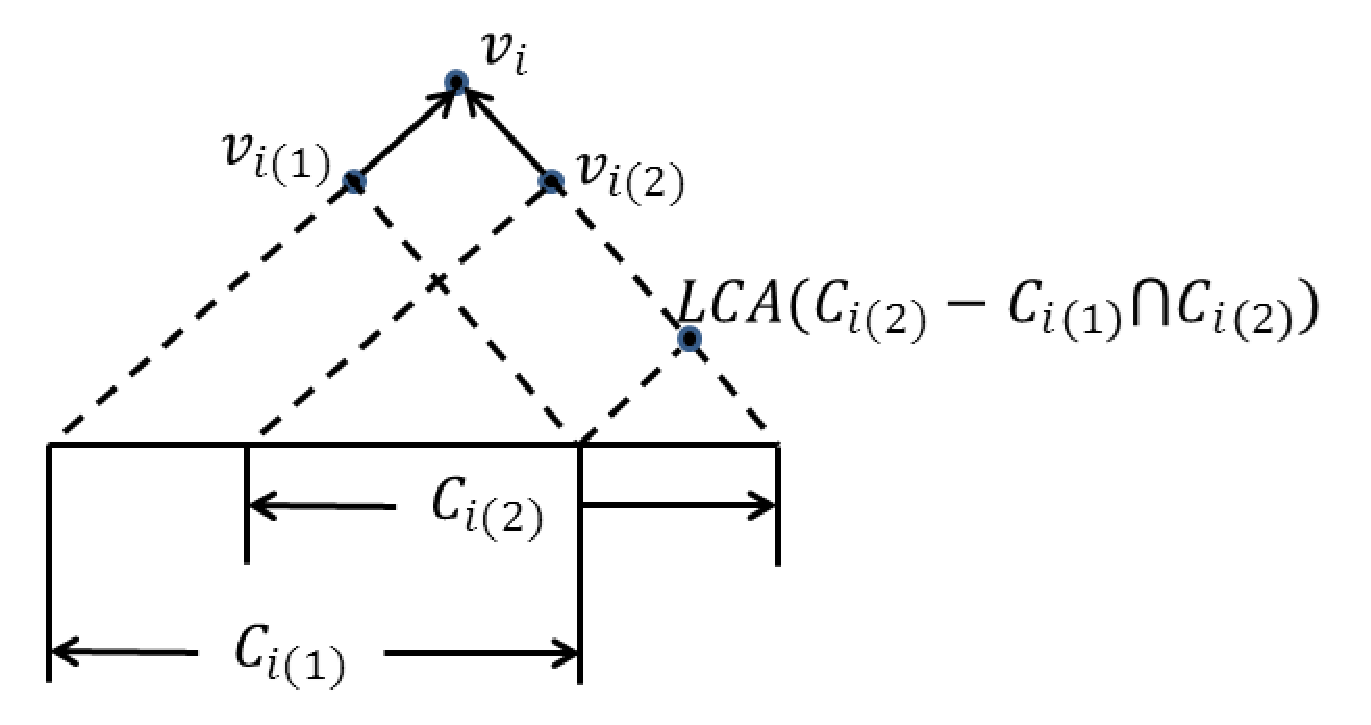
\includegraphics[scale=0.3]{figures/dag-overlap.eps}
\caption{Illustration of how to handle overlap}
\label{fig:dag-overlap}
\end{minipage}
\end{figure}

%This new algorithm adopts Charles' mechanism of FIFO to generate all
%unified columns
\begin{itemize}
    \item Prepare $g+1$ bins, i.e. $\{0, 1, \ldots, g\}$. Each bin $i$
    ($i \in [0, g]$) will correspondingly contains all columns that
    derived from original $m$ input columns and have $i$ ``x''s.

    \item Prepare a {FIFO} queue and put all initial $m$ input columns 
    into the {FIFO} queue. 

    \item Each time, remove a head element (column) from the {FIFO}
    queue, apply it with $\otimes$ operation to the rest of elements
    (columns) in the {FIFO} and insert resulting unified elements (columns)
    into the {FIFO} queue. After applying the head element to all
    the rest elements in {FIFO}, insert the head element into bin $i$
    according to how many ``x'' it has in it form.

\end{itemize}

\begin{theorem}
If assuming the number of initial input columns is $m$, the number of
total resulting unified (by $\otimes$ operation) but different columns
is $M$, then the total number of $\otimes$ operation is at most $O(M^2)$.
\label{thm:totalNodes}
\end{theorem}

\begin{IEEEproof}
Since the total number of elements (columns) in the {FIFO} queue is at
most $M$ at any moment, and each element will $\otimes$ with the rest
of elements in {FIFO} queue, so it's at most $O(M^2)$ times.
\end{IEEEproof}

\punt{%
    %for this old version, the conjecture that we only need to merge
    %columns in the same bin to produce all possible combinations of
    %medians (unified columns) is NOT true
\begin{itemize}

    \item Prepare $g+1$ bins, i.e. $\{0, 1, \ldots, g\}$. Each bin $i$
    ($i \in [0, g]$) will correspondingly contains all columns that
    derived from original $m$ input columns and have $i$ ``x''s.

    \item Initially, assuming all columns contain no ``x''s so that
    we put all nodes into bin $0$.

    \item Merge all ${m \choose 2}$ possible pairs in bin $0$, spread
    resulting nodes into bins $1, 2, \ldots, g$, respectively, according
    to the number of ``x''s appeared in merged nodes. E.g. if we merge
    column $(0, 1, 0)^T$ and column $(0, 1, 1)^T$, we get a new node
    $(0, 1, x)^T$ and it will go into bin $1$. If we merge node $(0,
    1, 0)^T$ and node $(0, 0, 1)^T$, we get a new node $(0, x, x)^T$
    and it should go to bin $2$, and so on.  In addition, for each node
    $v_i$, we associate it with a tuple $(\mathcal{C}_i, h_i)$, where
    $\mathcal{C}_i$ is the set of original input nodes that are leaves of
    the sub-tree rooted at node $v_i$, $h_i$ is the height of node $v_i$
    and equals to the number of ``x''s appeared in the new node.

    \item Since every non-leaf node is merged from two nodes in the lower
    level bins, if more than $1$ pair of nodes merged into the same node,
    we make a phantom node (see~\figref{phantom-node}), which has the same
    node signature, so as to make each node in the hierarchical {DAG}
    has two and only two children. It's easy to prove that if the old {DAG} 
    has $M$ nodes in total, after augmenting with phantom nodes, the new 
    {DAG} will have $\leq 2M$ nodes. Basically, the idea is to transform
    a non-binary tree to a binary tree by augmenting with phantom nodes.

    \item For bin $i$, we merge all ${bin(i) \choose 2}$ node
    combinations , spread the resulting nodes to bin $i+1, i+2, \ldots,
    g$, respectively, depending on the number of ``x''s appeared
    in merged nodes. Any collision of new nodes in any bins will be
    discarded due to redundancy.  We have the observation
    that for the ``merge'' operation, properties of idempotence, 
    associativity, and commutativity hold,
    i.e., for any node in bin $i$ that merged from input columns $\id{c_0},
    \id{c_1}, \ldots, \id{c_i}$, can be generated from two nodes
    in bin $i-1$ that merged from input columns $\id{c_0}, \id{c_1},
    \ldots, \id{c_{i-1}}$, and input columns $\id{c_1}, \id{c_2},
    \ldots, \id{c_{i}}$, respectively.

    \item Repeat above procedure at most $g$ iterations or until no
    bins have any increments of new nodes. 

\end{itemize}
} %end punt

\subsecput{stage2}{Compute the $k$-medians out of the hierarchical {DAG}}
In stage $2$, we need to compute a $k$-medians on $T$.

\begin{itemize}

    \item Naively, ${bin(0) + bin(1) + \ldots + bin(g) \choose k}$
    will be our global optimum. But this method will yield complexity
    bound ${M \choose k} = O(M^k)$.

    \item Another way to compute the $k$-medians out of the hierarchical
    {DAG} is via dynamic programming. Following algorithm to compute
    $k$-medians on the hierarchical {DAG} is largely adapted from the
    algorithm in \cite{Tamir96}. The algorithm in \cite{Tamir96} computes
    $k$-medians on a tree with $n$ nodes in time $O(kn^2)$.  For trees,
    any two sub-trees don't overlap with each other, but for {DAG}s, any
    two sub-trees can overlap. So the innovation of following algorithm
    lies in mostly how to handle overlaps.

        \begin{itemize}
        
            \item Define $d(\mathcal{V}_j) = d(\mathcal{C}_j) =
            h_j \times \sum_{c_{j,i} \in \mathcal{C}_j} c_{j, i}$,
            where $h_j$ is the height / bin number of root node $v_j$,
            $\mathcal{C}_j$ is the set of all input columns that can
            be covered in tree $T_{v_j}$, and $c_{j, i}$ are elements
            of set $\mathcal{C}_j$.  Note that $\mathcal{C}_j$ is also
            the set of leaves of tree $T_{v_j}$

            \item Define $d(\mathcal{V}_i) \oplus d(\mathcal{V}_j) = d(\mathcal{C}_i) \oplus d(\mathcal{C}_j) = 
            h_i \times \sum_{c_{i, l_i} \in \mathcal{C}_i 
                      \wedge c_{i, l_i} \notin \mathcal{C}_j} c_{i, l_i} + 
     \min \{h_i, h_j\} \times \sum_{c_{l_o} \in \mathcal{C}_i \cap \mathcal{C}_j} c_{l_o} +
            h_j \times \sum_{c_{j, l_j} \in \mathcal{C}_j 
                      \wedge c_{j, l_j} \notin \mathcal{C}_i}$.

            \item Define $\otimes$ to be a bit-wise operation depending
            on truth table of~\figref{truth-table}. So, $\mbox{LCA}(v_i,
            v_j) = v_i \otimes v_j$.

            \item For each node $v_i$, an integer $q = 1, \ldots, k$,
            define $G(v_i, q)$ be the optimal value of the subproblem
            defined on the sub-tree $T_{v_i}$, given that a total of at
            least $1$ and at most $q$ nodes (medians) are selected in
            $T_{v_j}$. Of course, the function $G(v_i, q)$ is computed
            only for $q \leq |\mathcal{V}_i|$, where $|\mathcal{V}_i|$
            is the number of total nodes (not just input columns)
            contained in sub-tree $T_{v_i}$.

            \item Define $d(G(v_i, q)) = d(\mathcal{C}_{m_0}) \oplus
            \ldots \oplus d(\mathcal{C}_{m_{q-1}})$, where $m_0,
            \ldots, m_{q-1}$ are the $q$ medians selected in sets
            $\mathcal{V}_j$

        \end{itemize}


    \item following procedure employs dynamic programming technique
    to compute the function $G(v_j, q)$ bottom up the hierarchial
    {DAG} $T$

    \begin{itemize}

        \item Apparently for every node $v_i$ in $T$, we define 
        $G(v_i, 0) = \infty$.

        \item If $v_i$ is a leaf of $T$, then $G(v_i, 1) = 0$. 
        $G(v_i, q) = 0$, for any $q \geq 1$.

        \item If $v_i$ is a non-leaf of $T$, since every non-leaf
        has two and only two children, we denote $v_{i(1)}$ to be the
        left child and $v_{i(2)}$ to be the right child of $v_i$ 
        respectively. We have recurrence (see \figref{dag-overlap}):
        \begin{align}
        \begin{split}
        G(v_i, q) = \min \{ 
            \min_{\substack{
                       q_1 + q_2 = q\\
                        q_1 \leq |\mathcal{C}_{i(1)} - \mathcal{C}_{i(1)} \cap \mathcal{C}_{i(2)}|\\
                        q_2 \leq |\mathcal{C}_{i(2)}| }}
                  \{ d(G(\mbox{LCA}(C_{i(1)} - C_{i(1)} \cap C_{i(2)}), q_1)) \oplus 
                     d(G(v_{i(2)}, q_2))
                  \}\\
                      , \\
            \min_{\substack{
                       q_1 + q_2 = q\\
                        q_1 \leq |\mathcal{C}_{i(1)}|\\
                        q_2 \leq |\mathcal{C}_{i(2)} - \mathcal{C}_{i(1)} \cap \mathcal{C}_{i(2)}| }}
                  \{ d(G(v_{i(1)}, q_1))) \oplus 
                     d(G(\mbox{LCA}(C_{i(2)} - C_{i(1)} \cap C_{i(2)}, q_2))
                  \}\\
                      , \\
            d(\mathcal{V}_i) \oplus
            \min_{\substack{
                       q_1 + q_2 = q-1\\
                        q_1 \leq |\mathcal{C}_{i(1)} - \mathcal{C}_{i(1)} \cap \mathcal{C}_{i(2)}|\\
                        q_2 \leq |\mathcal{C}_{i(2)}| }}
                  \{ d(G(\mbox{LCA}(C_{i(1)} - C_{i(1)} \cap C_{i(2)}), q_1)) \oplus
                     d(G(v_{i(2)}, q_2))
                  \}\\
                      , \\
            d(\mathcal{V}_i) \oplus
            \min_{\substack{
                       q_1 + q_2 = q-1\\
                        q_1 \leq |\mathcal{C}_{i(1)}|\\
                        q_2 \leq |\mathcal{C}_{i(2)} - \mathcal{C}_{i(1)} \cap \mathcal{C}_{i(2)}|}}
                  \{ d(G(v_{i(1)}, q_1)) \oplus
                     d(G(\mbox{LCA}(C_{i(2)} - C_{i(1)} \cap C_{i(2)}), q_2))
                  \}\\
        \}
        \end{split}
        \label{eq:recG}
        \end{align}

        In recurrence \ref{eq:recG}, terms ``$ \min_{\substack{
                       q_1 + q_2 = q\\
                        q_1 \leq |\mathcal{C}_{i(1)} - \mathcal{C}_{i(1)} \cap \mathcal{C}_{i(2)}|\\
                        q_2 \leq |\mathcal{C}_{i(2)}| }}
                  \{ d(G(\mbox{LCA}(C_{i(1)} - C_{i(1)} \cap C_{i(2)}), q_1)) \oplus 
                     d(G(v_{i(2)}, q_2))
                  \}$''
                  and 
                  ``$ \min_{\substack{
                       q_1 + q_2 = q\\
                        q_1 \leq |\mathcal{C}_{i(1)}|\\
                        q_2 \leq |\mathcal{C}_{i(2)} - \mathcal{C}_{i(1)} \cap \mathcal{C}_{i(2)}| }}
                  \{ d(G(v_{i(1)}, q_1))) \oplus 
                     d(G(\mbox{LCA}(C_{i(2)} - C_{i(1)} \cap C_{i(2)}, q_2))
                  \}$''
        represent the case that all $q$ medians are selected in two sub-trees
        of the tree $T_i$. 

        Terms ``$d(\mathcal{V}_i) \oplus
            \min_{\substack{
                       q_1 + q_2 = q-1\\
                        q_1 \leq |\mathcal{C}_{i(1)} - \mathcal{C}_{i(1)} \cap \mathcal{C}_{i(2)}|\\
                        q_2 \leq |\mathcal{C}_{i(2)}| }}
                  \{ d(G(\mbox{LCA}(C_{i(1)} - C_{i(1)} \cap C_{i(2)}), q_1)) \oplus
                     d(G(v_{i(2)}, q_2))
                  \}$''
                  and 
            ``$d(\mathcal{V}_i) \oplus
            \min_{\substack{
                       q_1 + q_2 = q-1\\
                        q_1 \leq |\mathcal{C}_{i(1)}|\\
                        q_2 \leq |\mathcal{C}_{i(2)} - \mathcal{C}_{i(1)} \cap \mathcal{C}_{i(2)}|}}
                  \{ d(G(v_{i(1)}, q_1)) \oplus
                     d(G(\mbox{LCA}(C_{i(2)} - C_{i(1)} \cap C_{i(2)}), q_2))
                  \} $''
        represent the case that we select node $v_i$ as one of the 
        medians, and select the rest $q-1$ medians from two sub-trees.

    \end{itemize}
\end{itemize}

\subsecput{opt}{Proof of Global Optimality}
In this section, we are trying to prove that the $k$-medians got from
above algorithm are the global optimum.

\begin{theorem}
Let's denote $v_0$ to be the root of the {DAG} $T$, global $k$-median
optimum $G(v_0, k)$ can be given by any two non-overlapping sub-trees
which covers the entire set of $\mathcal{C}_0$ by recurrence
\ref{eq:recG}. That is, if $T_i$ and $T_j$ are two sub-trees of $T$,
$(\mathcal{C}_i \cup \mathcal{C}_j = \mathcal{C}_0) \wedge (\mathcal{C}_i \cap \mathcal{C}_j = \emptyset)$, then 
        $G(v_0, k) = 
            \min \{ \min_{\substack{
                       k_1 + k_2 = k\\
                        k_1 \leq |\mathcal{V}_i|\\
                        k_2 \leq |\mathcal{V}_j| }}
                  \{ d(G(v_i, k_1)) \oplus d(G(v_j, k_2)) \}
                      , 
            d(\mathcal{V}_0) \oplus
            \min_{\substack{
                       k_1 + k_2 = k-1\\
                        k_1 \leq |\mathcal{V}_i|\\
                        k_2 \leq |\mathcal{V}_j| }}
                  \{ d(G(v_i, k_1)) \oplus d(G(v_j, k_2)) \}
        \}$. In short, let's denote $G(v_0, k) = \min_{k_1 + k_2 = k}\{ \mathcal{C}_i \odot \mathcal{C}_j \}$
\end{theorem}

\begin{IEEEproof}
Let's prove the theorem by induction on the height $h$ of the {DAG}:

\begin{itemize}
\item When height of {DAG} equals $0$, i.e. $v_0$ is a leaf node, apparently
$G(v_0, q)$, where $q \in [0, k]$ gives the global optimum.

\item When height of {DAG} equals $1$, which means, for non-leaf node $v_0$,
its only two sub-trees are leaves. Since it's binary tree and both its
sub-trees are leaves and non-overlapping, $G(v_0, q)$,
where $q \in [0, 3]$ gives the global optimum.

\item Assuming that for any {DAG} of height $h$, the conclusion holds.

\item For {DAG} $T_0$ of height $h+1$. If we divide $\mathcal{C}_0$ into
two disjoint sub-sets $\mathcal{C}_i$ and $\mathcal{C}_j$, apparently,
the corresponding $G(v_i, k_1)$, where $k_1 \leq |\mathcal{V}_i|$, 
and $G(v_j, k_2)$, where $k_2 \leq |\mathcal{V}_j|$ gives corresponding 
global optimum of two sub-trees $T_i$ and $T_j$. Now, we are going to 
prove that $G(v_0, k) = \min_{k_1 + k_2 = k}\{ \mathcal{C}_i \odot \mathcal{C}_j \}$ gives the global optimum of tree $T_0$. 

        Suppose it's not, which means that at least there is one median
        $m_k$ not in sub-trees $T_i$ or $T_j$. Since $\mathcal{C}_i \cup \mathcal{C}_j = \mathcal{C}_0$, so we can divide the input column set $\mathcal{C}_{m_k}$ of $T_{m_k}$ into two disjoint sets $\mathcal{C}_{m_k, i}$ and $\mathcal{C}_{m_k, j}$,
        such that $(\mathcal{C}_{m_k, i} \cup \mathcal{C}_{m_k, j} = \mathcal{C}_{m_k}) \wedge (\mathcal{C}_{m_k, i} \subseteq \mathcal{C}_i) \wedge (\mathcal{C}_{m_k, j} \subseteq \mathcal{C}_j)$. So, we can further divide $\mathcal{C}_i$
        into two sub-sets $\mathcal{C}_{m_k, i} \cup (\mathcal{C}_i - \mathcal{C}_{m_k, i})$, and divide $\mathcal{C}_j$ into two sub-sets $\mathcal{C}_{m_k, j} \cup (\mathcal{C}_j - \mathcal{C}_{m_k, j})$, respectively.

        According to the inductive hypothesis, $G(v_{m_k}, k) = \min_{k_1 + k_2 = k} \{ \mathcal{C}_{m_k, i} \odot \mathcal{C}_{m_k, j}\}$, 
        $G(v_i, k) = \min_{k_1 + k_2 = k}\{\mathcal{C}_{m_k, i} \odot (\mathcal{C}_{i} - \mathcal{C}_{m_k, i})\}$,
        $G(v_j, k) = \min_{k_1 + k_2 = k}\{\mathcal{C}_{m_k, j} \odot (\mathcal{C}_{j} - \mathcal{C}_{m_k, j})\}$.
        So, any benefits can be got from median $m_k$ must be already
        covered by two non-overlapping sub-trees $T_i$ and $T_j$.
\end{itemize}
\end{IEEEproof}
